\documentclass[a4paper,12pt]{article}
\usepackage[utf8]{inputenc}
\usepackage[english]{babel}
\usepackage{authblk}
\usepackage{graphicx}
\usepackage{mathptmx}
\usepackage[singlespacing]{setspace}
\usepackage[headheight=1in,margin=1in]{geometry}
\usepackage{fancyhdr}
\usepackage{lipsum}


\renewcommand{\headrulewidth}{0pt}
\pagestyle{fancy}


\makeatletter
\def\@maketitle{%
  \newpage

  \begin{center}%
  \let \footnote \thanks
    {\LARGE \@title \par}%
  \end{center}%
  \par
  \vskip 0.1em}
\makeatother

\chead{%
  $11$$^{th}$ International Conference on Computational Social Science IC$^{2}$S$^{2}$\\
  July 21-24, 2025, Norrköping, Sweden%
}

\graphicspath{{images/}}

\title{Developing a Large Language Model System for Swiss Cases on Choice of Law}

 
\date{}

\begin{document}

\maketitle
\thispagestyle{fancy}

\begin{center}
\textit{Keywords: NLP, LLMs, LLM Evaluation, Court Decisions, Private International Law}
\newline
\end{center}

\section*{Extended Abstract}

Introduction

Based on a data sample of 33 cases on choice of law, this study describes the development of a customized Large Language Model (LLM) system for private international law. The LLM system is equipped to handle three languages (German, French, and Italian) and handles expert input in English. This mirrors - on a small scale - the multilingual challenges encountered in our field.

The goal of this machine-learning experiment is to obtain high-quality legal analyses from the LLM system in four key categories: Relevant facts, choice of law issue, relevant rules of law, and court's position. The research endeavor is centered around determining if it is possible for LLMs to produce analyses comparable to those of legal professionals. Furthermore, it will be assessed to what extent an automated evaluation can contribute to determining the quality of the LLM-generated outputs.

OpenAI's XXX model, a pre-trained language model, is the primary model employed in this experiment. It uses advanced vectorization and embedding techniques. However, can this numerical representation capture the nuanced reasoning of case law interpretation?

- explain Court Decision Analysis for CoL
A standard case law brief can be seen as a general synthesis based on an official court document. A concise yet informative case law brief helps practioners, students, and scholars, by condensing pages of information into paragraphs. 

	- explain JD differences and why they matter
It is important to note that only a small fraction of cases can be considered 'PIL cases', e.g., cases where the core dispute explicitely refersto 'party autonomy' and the PIL problem is further elaborated in the decision. In general, PIL aspects often appear in disguise during court proceedings handling foreign elements.
  - explain original procedure with human evaluation
The analysis of a PIL case requires the nuanced differentiation between the merits of the dispute, which usually structures the entire court decision, and the PIL aspects, usually mentioned only en passant. These parenthetic aspects however, are the primary focus of a PIL analysis. Concretely, what a PIL-interested legal person is interested in are the following categories: (1) the section of the text dealing with the methodological choice of law issue, (2) the abstract of the case, (3) the relevant facts, (4) the private international law provisions used in the PIL argumentation, (5) the types of choice of law issues dealt with, (6) the actual choice of law issue phrased as a question, and (7) the court's position on the choice of law issue.

In a first installment of the experiment, the automated answers were generated and then given to a human legal expert for evaluating each court decision and each answering category with a previously defined set of evaluation metrics. The legal expert also made notes on specific intricacies they could identify from reading the automatically generated answers. This (timely!) effort allows for a particularly nuanced insight into the performance of the LLM. On a larger scale it quickly becomes inefficient/expensive to have every answer generated by an LLM reviewed by a human.

- explain goal of comparing evaluation methods

Thus, an automated evaluation approach might prove useful. To figure out the trustworthiness of such automated approaches, human evaluation, BERTscore, and G-Eval are computed and compared. During the human evaluation a legal export carefully rates each answer usually by accuracy and conciseness. Depending on the specific answering category, small adjustments are made to the evaluation metrics. To help the legal expert with this task, they were provided with a ground truth dataset, containing the manually created analysis categories for each court decision that was analysed. The legal expert could then compare the model generated answers with answers that could be expected to be correct. BERTScore works in a similar way. When computing the BERTScores, both ground truth and model generated answer are converted into BERT vector embeddings and then compared. The more similar the vectors are, the higher the returned score. G-Eval on the other hand does not require any additional data other than the model generated answer. G-Eval works by instructing an LLM to rate the quality of a given text by providing a prompt with detailed evaluation criteria. It is possible to break down this evaluation prompt into multiple steps. Because no additional data is required, G-Eval could be useful for instances, when cases are analysed that have never been sighted by a legal expert before. Not only could the process of creating answers be automated then, but if G-Eval proves trustworthy, an assessment of the quality of the generated answers can be provided too.

- explain goal of comparing different LLMs

- findings

The human evaluations proves that the generated answers reach a certain required standard for case law briefs. To determine the reliability of automated evaluation metrics, the correlation between BERTScore, G-Eval, and human evaluation scores was calculated. When comparing the scores returned from the automated evaluation with the human evaluation, it becomes clear that XXX. Fig X shows this and table X shows that.

\section*{References}
%...

\vskip 40pt
\underline {Guidelines:}
\begin{itemize}
\itemsep0pt
  \item 2 pages maximum (excluding references, figures and tables)
  \item Single spaced
  \item Font size 12pt
  \item 1-inch margins
  \item Do not include author names for blind review and remove any information that may identify the author(s)
\end{itemize}

\underline {Include in Order:}
\begin{itemize}
\itemsep0pt
  \item Paper title
  \item 5 keywords
  \item Extended abstract 
  \item References
  \item Figure or Table
\end{itemize}

\newpage

\begin{figure}[htp]
\centering
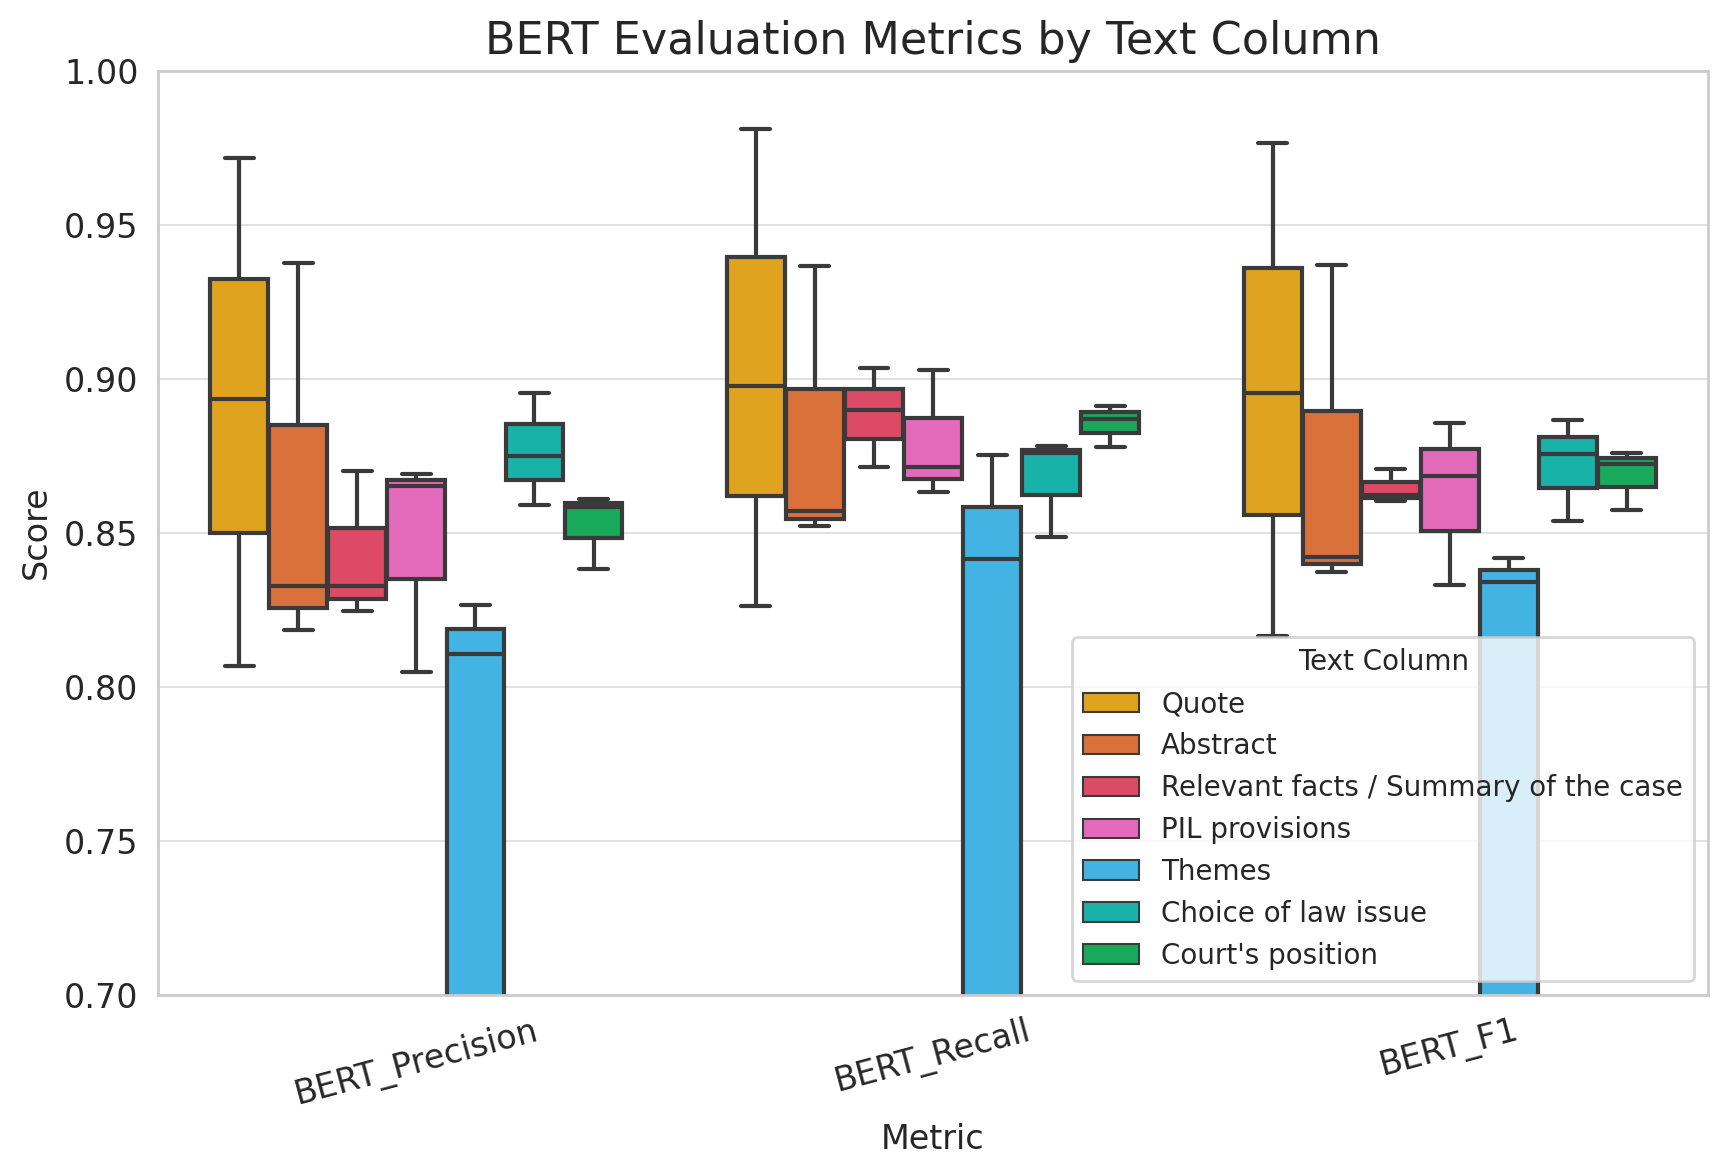
\includegraphics[width=14cm]{BERTScore-boxplots.png}
\caption{BERTScore evaluation metrics across all categories}
\label{fig:image}
\end{figure}

\end{document}
